% This text is proprietary.
% It's a part of presentation made by myself.
% It may not used commercial.
% The noncommercial use such as private and study is free
% Sep. 2005 
% Author: Sascha Frank 
% University Freiburg 
% www.informatik.uni-freiburg.de/~frank/
%
% additional usepackage{beamerthemeshadow} is used
%  
%  \beamersetuncovermixins{\opaqueness<1>{25}}{\opaqueness<2->{15}}
%  with this the elements which were coming soon were only hinted
%\documentclass[8pt]{beamer}
\documentclass[10pt]{beamer}
\usepackage{etex}
\newenvironment<>{varblock}[2][\textwidth]{%
  \setlength{\textwidth}{#1}
  \begin{actionenv}#3%
    \def\insertblocktitle{#2}%
    \par%
    \usebeamertemplate{block begin}}
  {\par%
    \usebeamertemplate{block end}%
  \end{actionenv}}
%\usepackage{hyperref}
%\usepackage{natbib}
%\usepackage{beamerthemeshadow}
\usepackage{beamerinnerthemecircles, beamerouterthemeshadow}

\usepackage{amsmath,amssymb,amsfonts}
\usepackage[pdf]{pstricks}
%\usepackage{bbm}
%\usepackage{booktabs}
\usepackage{amsthm}
\usepackage{booktabs}
\usepackage{graphicx}
\usepackage{epsfig}
%\usepackage{graphics}

% MQ: This is to be able to compile on the Riksbank computer. Uncomment with my laptop. Ugly solution but will have to do for now.
%\usepackage{epstopdf}
%\epstopdfsetup{outdir=./}

\usepackage{rotating}

\usepackage{url}
\usepackage{breqn}
%\usepackage{hyperref}
\usepackage[authoryear]{natbib}
\usepackage{setspace}
\usepackage{multirow}
%\usepackage{harvard}
\usepackage{xcolor}
%\usepackage{multicolumn}
\usepackage{algpseudocode}
\usepackage{sidecap}
\usepackage{bbm} 
\usepackage{courier}
\usepackage{tikz}
\usetikzlibrary{arrows,shapes,snakes,automata,backgrounds,petri}

\tikzset{
  treenode/.style = {align=center, inner sep=0pt, text centered,
    font=\sffamily},
  arn_n/.style = {treenode, circle, white, font=\sffamily\bfseries, draw=black,
    fill=black, text width=1.5em},% arbre rouge noir, noeud noir
  arn_r/.style = {treenode, circle, red, draw=red, 
    text width=1.5em, very thick},% arbre rouge noir, noeud rouge
  arn_x/.style = {treenode, rectangle, draw=black,
    minimum width=0.5em, minimum height=0.5em}% arbre rouge noir, nil
}
\beamertemplatenavigationsymbolsempty

\newenvironment{myenumerate}{\begin{enumerate}[(1)]}{\end{enumerate}} 
\sidecaptionvpos{figure}{c}
% FOR COLORING PARTS  OF TABLE
%\usepackage[beamer,customcolors]{hf-tikz}

%\tikzset{hl/.style={
%    set fill color=red!80!black!40,
%    set border color=red!80!black,
%  },
%}

\mode<presentation> {
    \usetheme{Madrid} %Frankfurt} %Bergen, Berkely, Berlin, Boadilla, CambridgeUS, Darmstadt,
                          %Frankfurt, Goettingen, Singapore, Warsaw
    \usecolortheme{beaver} %seahorse} %default} %beetle, seahorse, wolverine, dolphin, beaver
    %\useoutertheme[subsection=true]{smoothbars} 
    \usefonttheme{default}
    %\usecolortheme{red}
    

	\setbeamercolor{block title}{use=unstructure, fg=white, bg=purple!75!black} %{use=structure,fg=white,bg=purple!75!black}
	%\setbeamercolor{block body}{use=structure,fg=black,bg=white!20!white}    
    %\setbeamercolor{block body}{bg=white}
    \setbeamertemplate{enumerate items}[default]
    \setbeamercolor{enumerate item}{fg=purple!75!black} 
    \setbeamercolor{enumerate subitem}{fg=purple!75!black} 	 
	\setbeamercolor{itemize item}{fg=purple!75!black}  
	\setbeamertemplate{itemize item}[triangle]  
	\setbeamercolor{itemize subitem}{fg=purple!75!black}
	\setbeamertemplate{itemize subitem}[triangle]
	\setbeamertemplate{blocks}[framed]


}



%\usepackage{colortbl}
%\definecolor{yellow}{cmyk}{0,0.18,0.90,0.00}

%\usepackage{xcolor}

%\usepackage[authoryear]{natbib}
\begin{document}
\title[Lecture 7]{Bayesian Learning 732A46: Lecture 7}  
\author[Matias Quiroz]{Matias Quiroz\inst{1}$^{,}$\inst{2}}
\setbeamerfont{institute}{size=\fontsize{7pt}{8pt}}
\institute[LiU and Riksbank]{
  \inst{1}%
   Division of Statistics and Machine Learning, Link\"{o}ping University\\~\\
  \inst{2}%
   Research Division, Sveriges Riksbank\\
     
}

%\institute[Riksbank and LiU]{Sveriges Riksbank and Division of Statistics and Machine Learning, Link\"{o}ping University}

\date[]{April 2016} %\today 

%\usebackgroundtemplate{%
%  \vbox to \paperheight{\vfil\hbox to \paperwidth{\hfil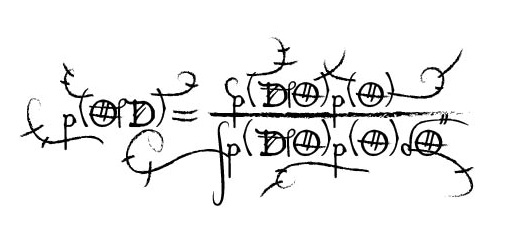
\includegraphics[width=1.5in]{Bayes.jpg}\hfil}\vfil}
%}

{
%\usebackgroundtemplate{\begin{center}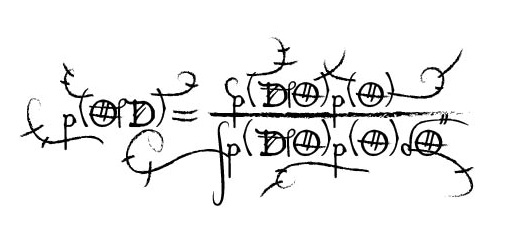
\includegraphics[width=0.4\paperwidth]{Bayes.jpg}\end{center}}
\usebackgroundtemplate{%
  \vbox to \paperheight{\hbox to \paperwidth{\hfil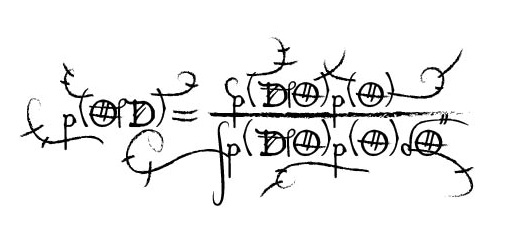
\includegraphics[width=2in]{Bayes.jpg}\hfil}}
}
\begin{frame}
\titlepage
\end{frame}
}
%\frame{\titlepage} 

%\frame{\frametitle{Overview of the talk}\tableofcontents}


\begin{frame}
\frametitle{Lecture overview}

\begin{itemize}
\item Bayesian computations - a recap
\bigskip
\item Grid based methods and their curse
\bigskip
\item Monte Carlo integration
\bigskip
\item First tools to simulate from unknown distributions

\end{itemize}

\end{frame}


\begin{frame}
\frametitle{Bayesian computations - a recap}

\begin{itemize}
\item The two \textbf{major steps} of any Bayesian analysis
\begin{enumerate}
\item[(1)] Obtain the posterior distribution.
\item[(2)] Average some function over the posterior distribution.
\end{enumerate}
\item[(1)] The {\color{blue}\textbf{posterior distribution}} $p(\theta|y)=p(\theta|y)$ by {\color{blue}Bayes' theorem} $$p(\theta|y) = \frac{p(y|\theta)p(\theta)}{p(y)} \propto p(y|\theta)p(\theta),\quad p(y)=\int p(y|\theta)p(\theta)d\theta.$$
\item For \textbf{{\color{blue}conjugate priors}} $p(\theta|y)$ is a {\color{blue}known distribution}. Only available for few and simple models.
\item[(2)] {\color{blue}Examples} [$\theta \sim \pi(\cdot)$ continuous. Replace $\int$ by $\sum$ for discrete $\theta$]
\vspace{1mm}
\begin{itemize}
\item[] {\color{blue}Expectation}: $E[\theta]=\int\theta p(\theta|y)d\theta$
\vspace{1mm}
\item[] {\color{blue}Prediction} : $p(\tilde{y}|y)=\int p(\tilde{y}|\theta) p(\theta|y)d\theta$
\vspace{1mm}
\item[] {\color{blue}Probabilities}: $\Pr(\theta \in A)=\int_A p(\theta|y)d\theta$. E.g. if $\theta \in [0,\infty)$ then $\Pr(\theta\leq 2)=\int_0^{2}p(\theta|y)d\theta$.
\end{itemize}
%\item So far we have derived $p(\theta|y)$ analytically. {\color{red}Cumbersome task} even for simplistic models. 
%\item This course module provide

\end{itemize}

\end{frame}

\begin{frame}
\frametitle{{\color{blue}Recall:} Nothing but expectations of a function}

\begin{itemize}
\item The examples in {\color{purple!75!black}(2)} are special cases of $$E[h(\theta)]=\int h(\theta)p(\theta|y)d\theta.$$
\item[] {\color{blue}Expectation}: $E[\theta]=\int\theta p(\theta|y)d\theta$. {\color{red} $h(\theta)=\theta$}.
\vspace{1mm}
\item[] {\color{blue}Prediction} : $p(\tilde{y}|y)=\int p(\tilde{y}|\theta) p(\theta|y)d\theta$. {\color{red} $h(\theta)=p(\tilde{y}|\theta)$}.
\vspace{1mm}
\item[] {\color{blue}Probabilities}: $\Pr(\theta \in A)=\int_A p(\theta|y)d\theta = \int \mathbbm{1}_A(\theta)p(\theta|y)d\theta$. {\color{red} $h(\theta)=\mathbbm{1}_A(\theta)$}, $${\color{red}\mathbbm{1}_A(\theta)} = \left\{\begin{array}{ll}1, \textnormal{ if } \theta \in A,\\
0, \textnormal{ if } \theta \notin A,
\end{array}\right.$$
\item {\color{red}Note}: the function of interest is \textbf{{\color{blue}averaged over the posterior uncertainty}} of the parameters. 
\end{itemize}

\end{frame}


\begin{frame}
\frametitle{Grid-based solution to compute $E[h(\theta)]$}
\begin{itemize}
%\item Numerical integration
%\begin{enumerate}
%\item {\color{blue}Grid-based methods}.
%\item Simulation methods.
%\end{enumerate}
\item Consider $\theta \in \mathbb{R}$ and form \textit{a grid} $$\theta^{g} = (\theta^{(1)}, \theta^{(2)}, \dots, \theta^{(S)}),$$
where $\theta^{(1)} < \theta^{(2)} < \dots < \theta^{(S)}$. 
\item {\color{blue}Important}: the grid {\color{blue}covers the parameter space} where $h(\theta) p(\theta|y) \neq 0$. The expectation is
%\item[] \noindent
\small{\begin{eqnarray*}
E[h(\theta)] &=&\int_{\theta^{(1)}}^{\theta^{(S)}} h(\theta) p(\theta|y)d\theta \\
 & = & \int_{\theta^{(1)}}^{\theta^{(2)}} h(\theta) p(\theta|y)d\theta + \int_{\theta^{(2)}}^{\theta^{(3)}} h(\theta) p(\theta|y)d\theta + \dots + \int_{\theta^{(S-1)}}^{\theta^{(S)}} h(\theta) p(\theta|y)d\theta
\end{eqnarray*}} \normalsize
%\begin{multline*}
%E[h(\theta)]=\int_{\theta^{(1)}}^{\theta^{(S)}} h(\theta) p(\theta|y)d\theta \\ =  \int_{\theta^{(1)}}^{\theta^{(2)}} h(\theta) p(\theta|y)d\theta + \int_{\theta^{(2)}}^{\theta^{(3)}} h(\theta) p(\theta|y)d\theta + \dots + \int_{\theta^{(S-1)}}^{\theta^{(S)}} h(\theta) p(\theta|y)d\theta
%\end{multline*}
\item Let $f(\theta) = h(\theta)p(\theta|y)$, $$\int_a^b f(\theta)d\theta \approx \text{\color{blue}The area under the curve } f(\theta) \text{ \color{blue}    between \textit{\color{red}a} and \textit{\color{red}b}}.$$  
\end{itemize}

\end{frame}

\begin{frame}
\frametitle{Grid-based solution to compute $E[h(\theta)]$, cont.}
\begin{itemize}
\item Some simple {\color{blue} quadrature} rules ({\color{blue}quadrature} = \textit{\textbf{determining area} in Latin})
\begin{itemize}
\item $\int_a^b f(\theta)d\theta \approx (b-a)f(\frac{a+b}{2})$. {\color{blue}Midpoint rule}. A {\color{red}constant} interpolation.
\item $\int_a^b f(\theta)d\theta \approx (b-a)\frac{f(a)+f(b)}{2} $. {\color{blue}Trapezoidal rule}. A {\color{red}linear} interpolation.
\end{itemize}
\item {\color{blue}Simpson's rule} is obtained with a {\color{red}quadratic} interpolation.
%\item Choose the grid adaptively can give better approximations. 
\item R routines: \texttt{gaussquad, integrate} (1 dim), \texttt{adaptIntegrate} (multi-dimensional).
\item Grid-based methods are {\color{red}cursed}. Consider $\theta \in \mathbb{R}^p$ and create a grid for each parameter
\begin{eqnarray*}
\theta_1^{g} & = & (\theta_1^{(1)}, \theta_1^{(2)}, \dots, \theta_1^{(S_1)}) \\
& \vdots & \\
\theta_p^{g} & = & (\theta_p^{(1)}, \theta_p^{(2)}, \dots, \theta_p^{(S_p)}).
\end{eqnarray*}
\item The {\color{blue}meshed grid} is the tensor product $\theta_1^{g}\times \theta_2^{g} \times \dots \times \theta_p^{g}$.
\item Grows {\color{red}exponentially}. {\color{blue}Example}: If $p=5$, then $100$ grid point in each dimension $\rightarrow 100^5$ ({\color{red}10 billion}) points on the grid. \textbf{The curse of dimensionality.} 
\end{itemize}

\end{frame}


\begin{frame}
\frametitle{Simulation-based solution to compute $E[h(\theta)]$}
\begin{itemize}
\item {\color{blue}Monte Carlo} integration to the rescue.
\item Suppose we have {\color{red}iid.} draws $\{\theta^{(i)}\}_{i=1}^N$ from $p(\theta|y)$. By the {\color{blue}strong law of large numbers}
$$\frac{1}{N}\sum_{i=1}^N h(\theta^{(i)}) \xrightarrow{a.s} E[h(\theta)].$$
\item Because of the {\color{red}iid. property} I will refer to this as {\color{blue}non-Markovian} simulation.
\item Let $I$ denote the {\color{blue}expectation} (integral) $E[h(\theta)]=\int h(\theta)p(\theta|y)d\theta$. {\color{blue}We estimate} it by
$$\hat{I} = \frac{1}{N}\sum_{i=1}^N h(\theta^{(i)}), \quad \theta^{(i)} \stackrel{iid.}{\sim} p(\theta|y).$$ 
\item Note that $$V[\hat{I}] = \frac{\sigma^2}{N}, \quad \text{with } \sigma^2 = V[h(\theta^{(i)})]$$.
\item $V[\hat{I}]\rightarrow 0$ (provided $\sigma^2$ is bounded).  {\color{blue}Independent of the dimension of the integral} (the number of parameters $p$).
\end{itemize}

\end{frame}

\begin{frame}
\frametitle{Our friends revisited with Monte Carlo integration}
\begin{itemize}
\item Let $\{\theta^{(i)}\}_{i=1}^N$ be samples from $p(\theta|y)\propto p(y|\theta)p(\theta)$ ({\color{red} Does not have to be iid.})
\bigskip
\item {\color{blue}Expectation}: $E[\theta]\approx \frac{1}{N}\sum_{i=1}^N \theta^{(i)}$.
\bigskip
\item {\color{blue}Prediction} : $p(\tilde{y}|y)\approx \frac{1}{N}\sum_{i=1}^N p(\tilde{y}|\theta^{(i)}) $.
\bigskip
\item {\color{blue}Probabilities}: $\Pr(\theta \in A) \approx \frac{1}{N}\{\#\theta^{(i)} \text{ draws } \in A\}$.

\end{itemize}

\end{frame}


\begin{frame}
\frametitle{Simulation of unknown distributions}
\begin{itemize}
\item \textbf{If} we have samples it is (\textbf{\color{red}very}) easy to do \textbf{\color{blue}posterior inference}.\medskip
\item The challenge is to actually \textbf{obtain the samples}.\medskip
\item \textbf{Analytic derivations} used so far. \textbf{\color{red}Very cumbersome} - even for simplistic models. Often impossible.\medskip
\item We start with generating iid. (\textbf{\color{blue}non-Markovian}) samples.
\begin{enumerate}
\item The \textbf{\color{blue}inverse cdf} for a discrete distribution.
\item \textbf{\color{blue}Rejection sampling}.
\end{enumerate}
\medskip
\item \textbf{Note:} Everything I present is \textbf{general} for sampling from \textit{any distribution} (not necessarily the \textbf{\color{blue}posterior}).
\medskip
\item Since we are \textbf{\color{blue}Bayesians} I call the r.v. $\theta$ (the parameter) instead of $X$ which you can find in some literature.
\end{itemize}

\end{frame}


\begin{frame}
\frametitle{The inverse cdf method for a continuous distribution}
\begin{center}
\begin{minipage}{\columnwidth}
\begin{varblock}[0.8\columnwidth]{The inverse cdf for a continuous distribution}
Obtain $N$ samples from $F_\theta(\phi)=\Pr(\theta \leq \phi)$. Let $F^{-1}$ denotes the inverse.
\begin{itemize}
\item For $i=1, \dots, N$, repeat
\begin{enumerate}
\item $u\sim \texttt{uniform}(0,1)$
\item $\theta^{(i)} = F_{\theta}^{-1}(u)$
\end{enumerate}
\end{itemize}
\end{varblock}
\end{minipage}
\end{center}
%\begin{itemize}
%\item \textbf{Proof:}
\begin{proof}[{\color{yellow}Proof that we get the correct distribution for $\theta$}]
$\Pr(\theta \leq \phi)  =  \Pr(F_{\theta}^{-1}(u) \leq \phi)=\Pr(u \leq F_{\theta}(\phi))= F_{\theta}(\phi).$
\\ This means that $$\theta \sim F_{\theta}.$$
\end{proof}
%\end{itemize}

\end{frame}


\begin{frame}
\frametitle{The inverse cdf for a discrete distribution}
\begin{itemize}
\item Useful as a \textbf{\color{blue}discrete approximation} of a continuous $\theta$.
\end{itemize}
\begin{center}
\begin{minipage}{\columnwidth}
\begin{varblock}[0.8\columnwidth]{The inverse cdf for a discretized continuous variable}
Obtain $N$ samples from $p(\theta|y)$ known up to a normalizing constant, $\theta \in \mathbb{R}.$
\begin{itemize}
\item \textbf{Evaluate} $p(y|\theta_j)p(\theta_j)$ for each $$\theta_j \in  (\theta_1, \theta_2, \dots, \theta_S) \quad (\text{\color{red}a dense grid}).$$
\item \textbf{Normalize} $\hat{f}_j = p(y|\theta_j)p(\theta_j)/\sum_{l=1}^S p(y|\theta_l)p(\theta_l).$
\item \textbf{Compute} the empirical cdf (cumulative sum) $\hat{F}$ of $\hat{f}=(\hat{f}_1, \dots, \hat{f}_S).$
\item For $i=1, \dots, N$, repeat
\begin{enumerate}
\item $u\sim \texttt{uniform}(0,1)$
\item $\theta^{(i)} = \hat{F}^{-1}(u)$
\end{enumerate}
\end{itemize}
\end{varblock}
\end{minipage}
\end{center}
\begin{itemize}
\item \textbf{Drawback}: a grid, \textbf{\color{red}computationally intractable} for a couple of dimensions.
\item Useful for simulating \textbf{parts of the posterior} that are {\color{blue}one dimensional}. 
\end{itemize}

\end{frame}


\frame{\frametitle{Example of inverse cdf on a discrete sample space $\{0,2,5\}$}

\begin{figure}[H]
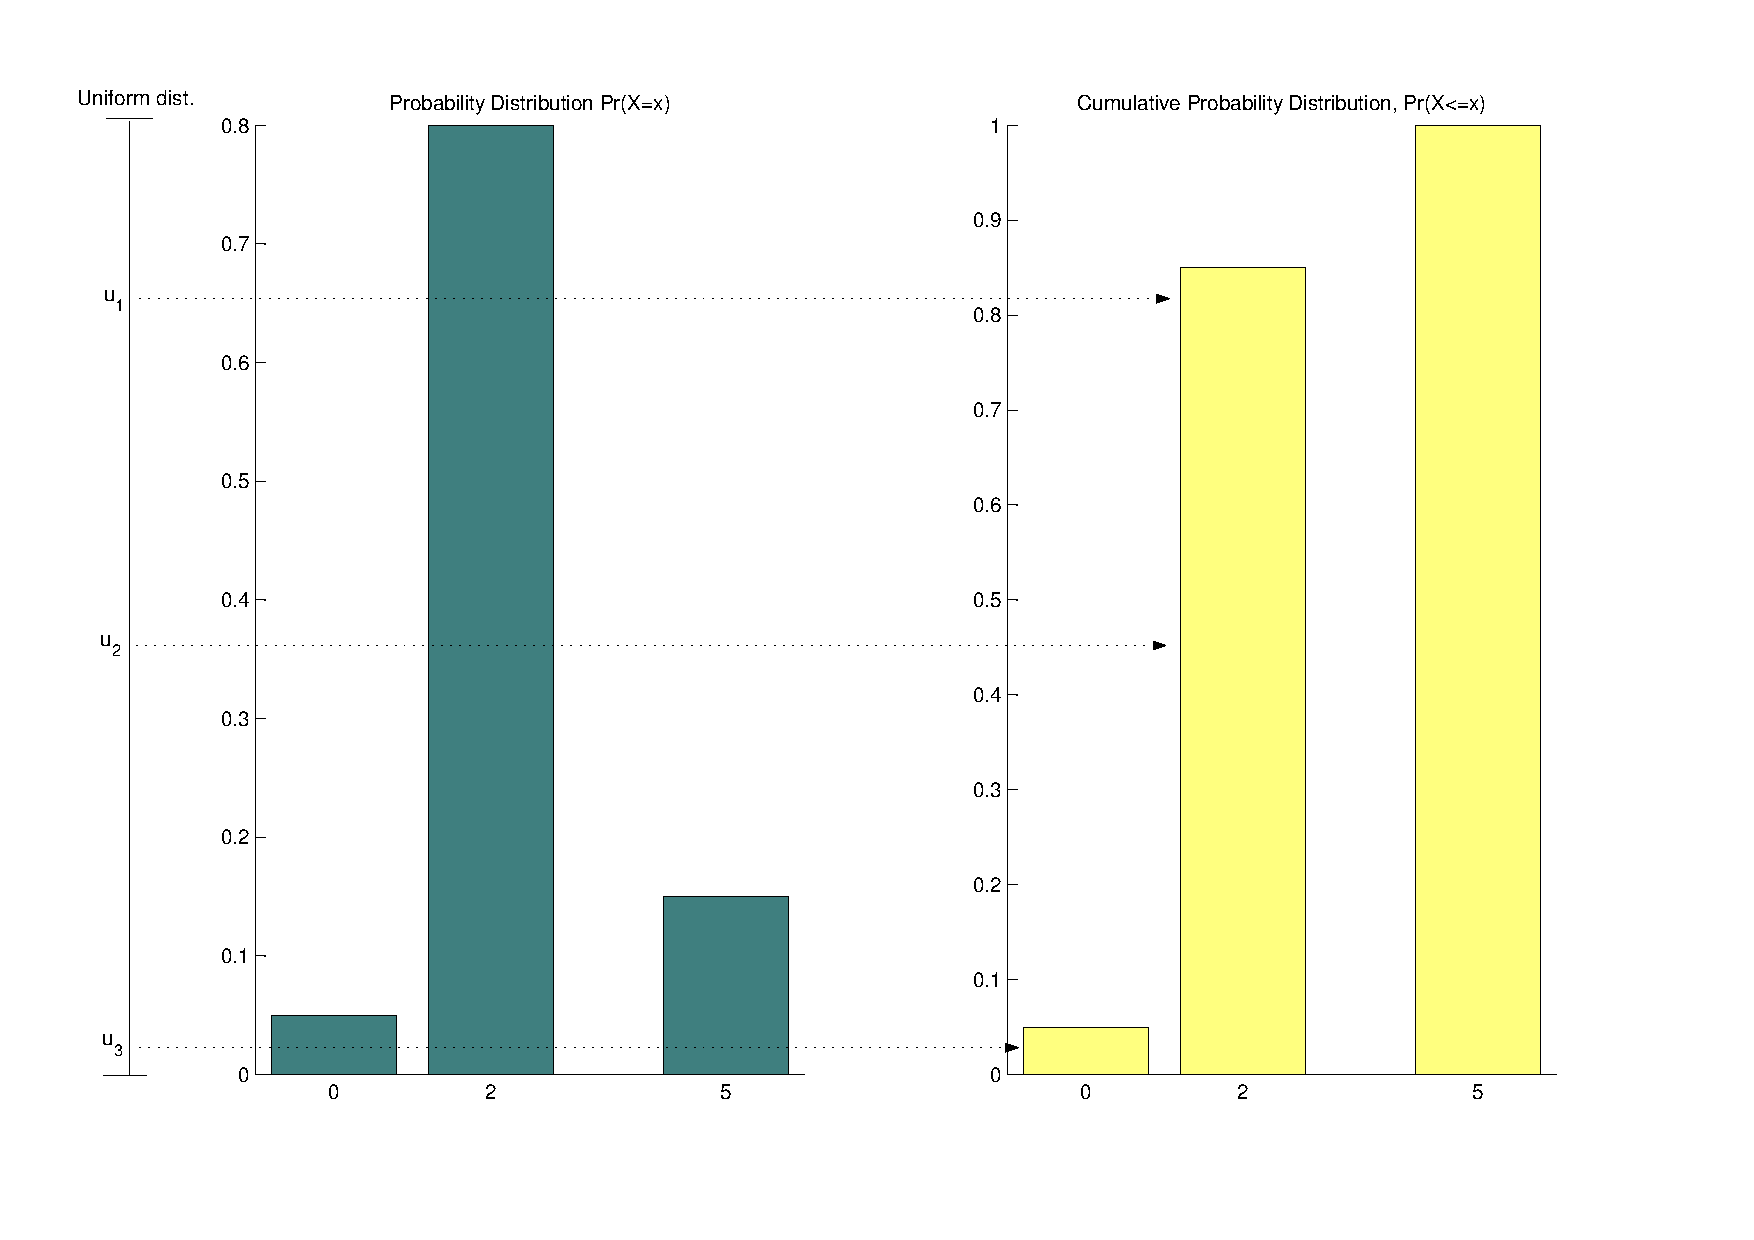
\includegraphics[width=\columnwidth]{InverseCDF}
%\protect\caption{$\p(\alpha, \beta|y)$}
\end{figure}
}

\begin{frame}
\frametitle{Recall: Estimating the shrinkage parameter $\lambda$}
\begin{itemize}
\item The normal regression model with \textbf{\color{blue}unknown shrinkage}
$$y=X\beta +\varepsilon, \quad \varepsilon \in \mathcal{N}(0, \sigma^2 I)$$
%\item $y \sim \mathcal{N}(X\beta, \sigma^2 I}$

\item The \textbf{joint posterior} (see priors below) factorizes $$p(\beta,\sigma^2,\lambda|y) = p(\beta|\sigma^2,\lambda,y)p(\sigma^2|\lambda,y)p(\lambda|y),$$\\
\begin{tabular}{rcl}
$\textbf{\color{blue}Prior} \quad\quad\quad$ &  $\rightarrow$ & 
\vspace{3mm}
$\quad\quad\quad\textbf{\color{blue}Posterior}$ \\
\vspace{3mm}
$\beta | \sigma^2, \lambda \sim \mathcal{N}(0,\sigma^2\Omega_0^{-1})$ & $\rightarrow$ & $\beta|\sigma^2, \lambda, y \sim  \mathcal{N}(\beta_n, \sigma^2\Omega_n^{-1})$ \\
\vspace{2mm}
$\sigma^2 \sim \text{Inv-}\chi^2(\nu_0,s_0^2)$ & $\rightarrow$ & $\sigma^2 | \lambda, y \sim \text{Inv-}\chi^2(\nu_n,s_n^2)$ \\
$\lambda \sim p(\lambda)$ & $\rightarrow$ & $\lambda| y \sim  \sqrt{\frac{|\Omega_0 |}{|\Omega_n |}}\left(\frac{\nu_ns^2_n}{2}\right)^{-\nu_n/2} p(\lambda) $
\end{tabular}
\\~\\ and \\~\\
\begin{tabular}{ll}
$\beta_n  =  (X^{\prime}X+\Omega_0)^{-1}X^{\prime}y  $ & $\Omega_n = X^{\prime}X+\Omega_0 $ \\
$\nu_n = \nu_0 + n $ & $\nu_n s^2_n = \nu_0s^2_0+y^{\prime}y - \beta_n^{\prime}\Omega_n \beta_n$
\end{tabular}
\item $p(\lambda|y)$ \textbf{\color{blue}complex}. Can easily be evaluated on a grid! Inverse cdf to the rescue.
\end{itemize}
\end{frame}



\begin{frame}
\frametitle{Rejection sampling}
\begin{itemize}
\item \textbf{{\color{blue}The setting}}: 
\begin{itemize}
\item \textbf{Not possible to simulate} $p(\theta|y)\propto p(y|\theta)p(\theta)$ directly ({\color{red}not of known form}).
\item \textbf{We can bound} $p(y|\theta)p(\theta)\leq Mg(\theta), \quad \forall \theta$, where $M$ is \textbf{\color{blue}a constant} and $g(\theta)$ is a function with $\int g(\theta)d\theta <\infty$.
\item \textbf{We can sample} from a density proportional to $g(\theta)$. 
\end{itemize}
\end{itemize}
\pause
\begin{figure}[H]
\includegraphics[width=0.65\columnwidth]{RejectionSampling}
%\protect\caption{$\p(\alpha, \beta|y)$}
\end{figure}


\end{frame}



\begin{frame}
\frametitle{Rejection sampling, cont.}

\begin{center}
\begin{minipage}{\columnwidth}
\begin{varblock}[0.8\columnwidth]{Rejection sampling}
Obtain $N$ samples from $p(\theta|y)$ known up to a normalizing constant.\begin{itemize}
\item Set \texttt{i} = 1.
\item While \texttt{i} $\leq N$ do:
\begin{enumerate}
\item Generate a {\color{blue}candidate} $\theta^{\prime} \sim g(\theta)$.
\item Compute the {\color{blue}probality of acceptance} $$a = \frac{p(y|\theta)p(\theta)}{Mg(\theta)}\quad \text{\color{blue} and draw }u\sim \texttt{uniform}(0,1).$$
\item {\color{blue}If} $u\leq a\implies\theta^{(i)}=\theta^{\prime}$, {\color{blue}else} return to Step {\color{purple!75!black}1.}
\item \texttt{i} = \texttt{i} + 1.
\end{enumerate}
\end{itemize}
\end{varblock}
\end{minipage}
\end{center}

\end{frame}


\begin{frame}
\frametitle{Rejection sampling, cont.}
\begin{proof}[Conditional on acceptance, $\theta$ has density $p(\theta|y)$]
For \textbf{clarity and simplified} computations consider the ratio $\frac{p(\theta|y)}{Mg(\theta)}$.
{\small
\begin{eqnarray*}
\Pr\left(\theta \leq \phi | u \leq \frac{p(\theta|y)}{Mg(\theta)} \right) &= & \frac{\Pr\left(\theta \leq \phi , u \leq \frac{p(\theta|y)}{Mg(\theta)} \right)}{\Pr\left(u \leq \frac{p(\theta|y)}{Mg(\theta)} \right)} \\ 
& = & \frac{\int_{-\infty}^{\phi}\int_0^{\frac{p(\theta|y)}{Mg(\theta)} }g(\theta)dud\theta}{\Pr\left(u \leq \frac{p(\theta|y)}{Mg(\theta)} \right)} \\
& = & \frac{\int_{-\infty}^{\phi} \frac{p(\theta|y)}{Mg(\theta)}g(\theta)d\theta}{\int_{-\infty}^{\infty} \frac{p(\theta|y)}{Mg(\theta)}g(\theta)d\theta} \\
& = & \frac{\frac{1}{M}\int_{-\infty}^{\phi} p(\theta|y)d\theta}{\frac{1}{M}\int_{-\infty}^{\infty}  p(\theta|y)d\theta} = \int_{-\infty}^{\phi} p(\theta|y)d\theta. %\frac{\frac{p(y)}{p(y)}\int_{-\infty}^{\phi} p(y|\theta)p(\theta)d\theta}{p(y)} \\
%& = & \int_{-\infty}^{\phi} p(\theta|y)d\theta.
\end{eqnarray*}
}
\end{proof}
\end{frame}


\begin{frame}
\frametitle{Rejection sampling, cont.}
\begin{itemize}
\item \textbf{The density} $g(\theta)$ for \textbf{{\color{blue} unimodal cases}}:
\begin{itemize}
\item \textbf{Multivariate t} is a good choice. \textbf{Heavy tails} with low degrees of freedom. Let the mean and covariance matrix of $g(\theta)$ match those of the posterior. Use \texttt{optim} in R.
\item Choose $$M = \sup_{\theta} \frac{p(y|\theta)p(\theta)}{g(\theta)},$$ gives $a=1$ at the corresponding $\theta$.
\end{itemize} 
\item \textbf{{\color{blue}Multimodal posterior}}: Sample uniformly (at the cost of accepting fewer samples).
\item  \textbf{{\color{red} Drawbacks}} of rejection sampling:
\begin{enumerate}
\item If $g(\theta)$ is \textbf{\color{blue}"not so proportional"} to $p(y|\theta)p(\theta)$ \textbf{\color{red}few} draws are accepted.
\item In \textbf{\color{blue}high dimensions}: Difficult to find a good $M$ and $g(\theta)$ so that $p(y|\theta)p(\theta)\leq Mg(\theta)$. Making $M$ \textbf{too large} gives a \textbf{low} the probability of accepting a sample (\textbf{acceptance} $\propto \frac{1}{M}$).
\end{enumerate}
\item \textbf{\color{blue}A precursor} to the \textbf{{\color{blue}Metropolis-Hastings}} algorithm.
\end{itemize}
\end{frame}


%
%\begin{frame}{Lecture overview}
%
%\begin{itemize}
%\item \textbf{\textcolor{blue}{Monte Carlo simulation and random number
%generation\bigskip{}
%}}
%\item \textbf{\textcolor{blue}{Gibbs sampling\bigskip{}
%}}
%\item \textbf{\textcolor{blue}{Data augmentation}}
%
%\begin{itemize}
%\item \textbf{\textcolor{blue}{Probit regression}}
%\item \textbf{\textcolor{blue}{Mixture models}}
%\end{itemize}
%\end{itemize}
%\end{frame}
%
%\begin{frame}{Monte Carlo sampling}
%
%\begin{itemize}
%\item If $\theta^{(1)},\theta^{(2)},....,\theta^{(N)}$ is an \textbf{\textcolor{blue}{$iid$
%sequence}} from a distribution $p(\theta)$, then
%\begin{eqnarray*}
%\frac{1}{N}\sum_{t=1}^{N}\theta^{(t)} & \rightarrow & E(\theta)\\
%\frac{1}{N}\sum_{t=1}^{N}g(\theta^{(t)}) & \rightarrow & E[g(\theta)]
%\end{eqnarray*}
%where $g(\theta)$ is some well-behaved function.
%\item Easy to compute \textbf{tail probabilities} $\mathrm{Pr}(\theta\leq c)$
%by letting 
%\[
%g(\theta)=I\left(\theta\leq c\right)
%\]
%and 
%\[
%\frac{1}{N}\sum_{t=1}^{N}g(\theta^{(t)})=\frac{\#\text{ }\theta\text{-draws smaller than }c}{N}.
%\]
%
%\end{itemize}
%\end{frame}
%
%\begin{frame}{{\Large{}Direct sampling by the} {\Large{}inverse CDF\ method}}
%
%\begin{itemize}
%\item How to \textbf{\textcolor{blue}{simulate}} from a distribution?
%\item Let $f(x)$ be the density function of a stochastic variable. CDF:
%$F(x)$. \textbf{\textcolor{blue}{Inverse CDF\ method}}:
%
%\begin{enumerate}
%\item Generate $u$ from the uniform distribution on $[0,1]$.
%\item Compute $x=F^{-1}(u)$.
%\end{enumerate}
%\item Example 1: \textbf{Exponential} \textbf{distribution}: 
%\[
%u=F(x)=1-\exp(-\lambda x)
%\]
%Inverting gives
%\[
%x=-\ln(1-u)/\lambda
%\]
%But $1-u$ is also uniformly distributed on {[}0,1{]}. So:
%\item If $x=-(\ln u)/\lambda$ where $u\sim Unif(0,1)$, then $x\sim Expon(\lambda)$.
%\end{itemize}
%\end{frame}
%
%\begin{frame}{Inverse CDF method, discrete case}
%
%
%\begin{center}
%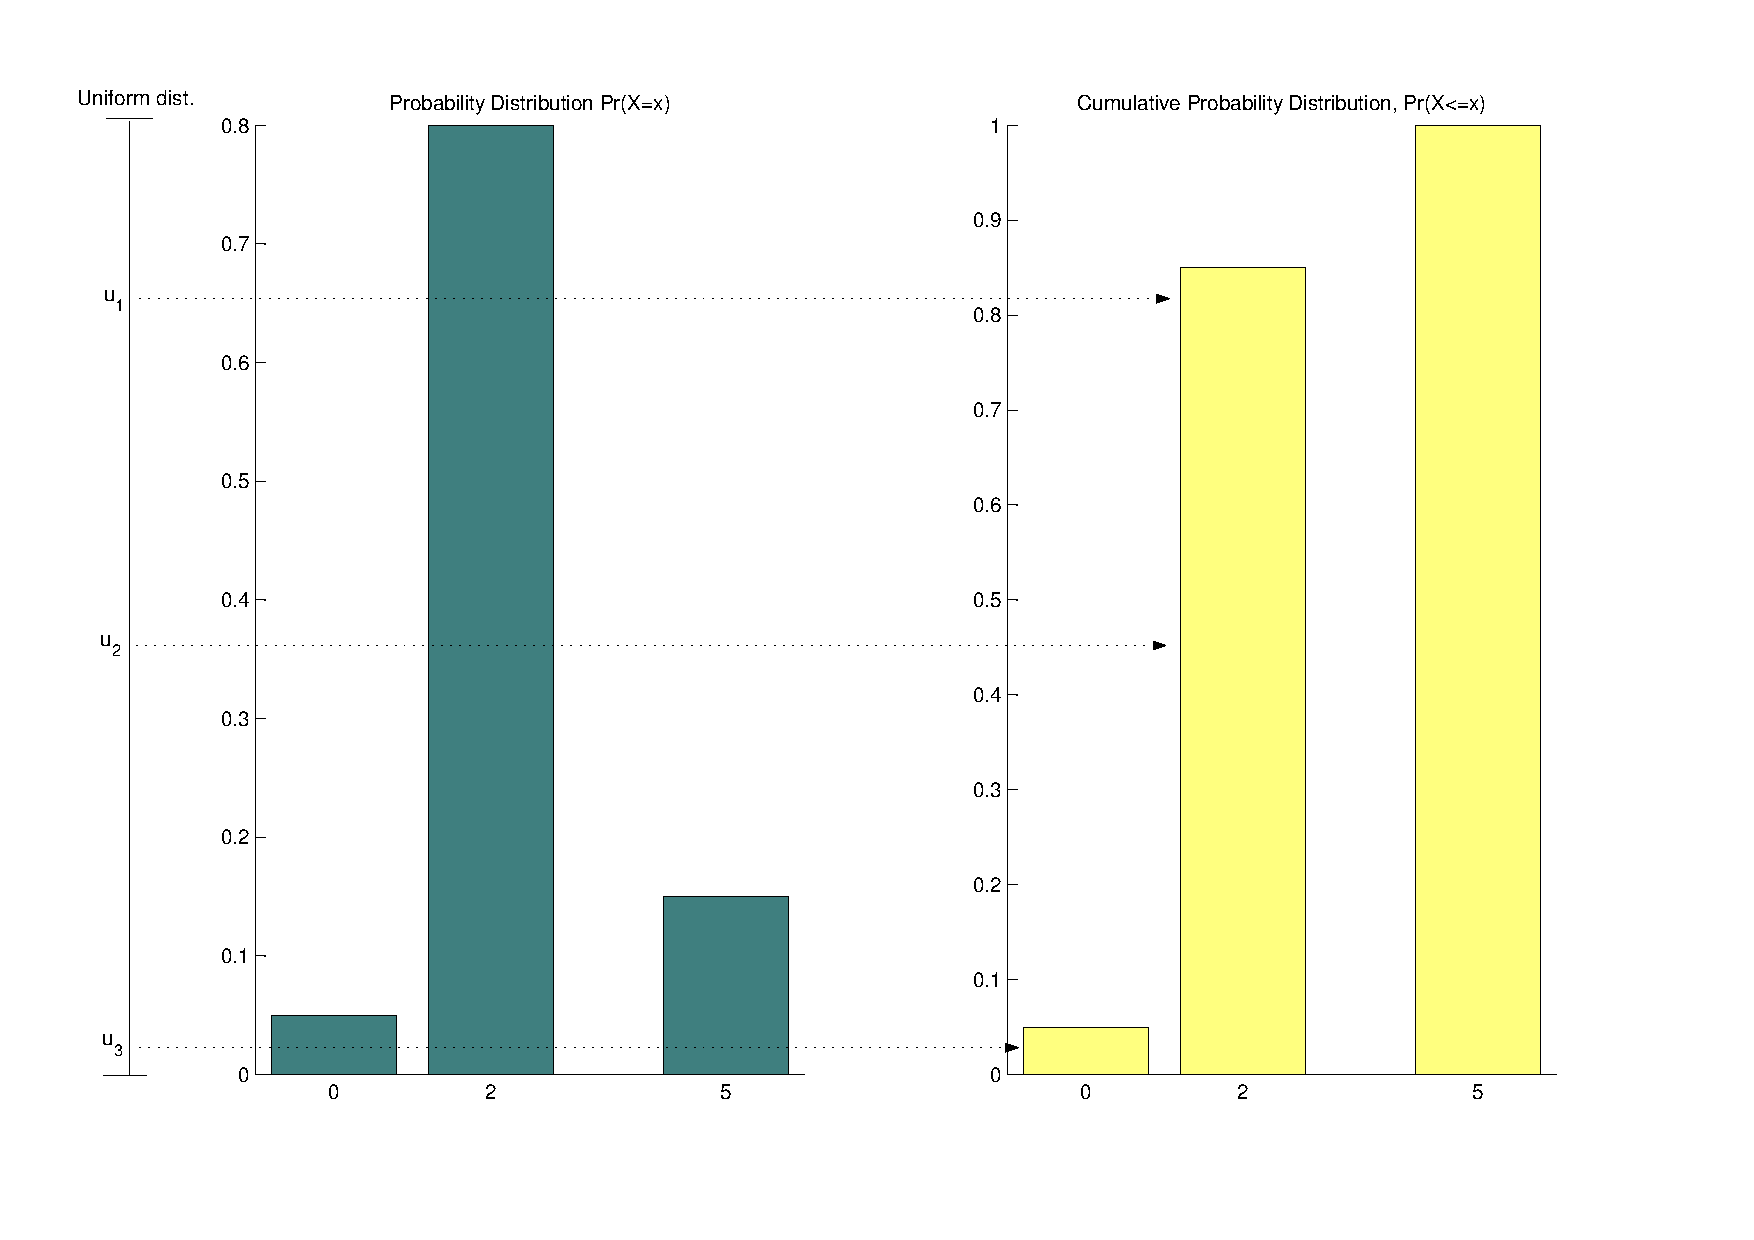
\includegraphics[scale=0.4]{InverseCDF}
%\par\end{center}
%
%\end{frame}
%
%\begin{frame}{{\Large{}Direct sampling by the} {\Large{}inverse CDF\ method}}
%
%\begin{itemize}
%\item Example 2: \textbf{\textcolor{blue}{Cauchy distribution}}: 
%\begin{eqnarray*}
%f(x) & = & \frac{1}{\pi}\frac{1}{1+x^{2}}\\
%u & = & F(x)=\frac{1}{2}+\frac{1}{\pi}\arctan(x)
%\end{eqnarray*}
%Inverting ...
%\[
%x=\tan[\pi(u-1/2)].
%\]
%
%\item We can also use relations between distribution to sample from distributions.
%\item Cauchy-example, cont. If $y$ and $z$ are independent $N(0,1)$ variables,
%then $z=\frac{y}{z}\sim Cauchy$.
%\item Example: \textbf{\textcolor{blue}{Chi-square}}. If $x_{1},...,x_{v}\overset{iid}{\sim}N(0,1)$,
%then $y=\sum_{i=1}^{v}x_{i}^{2}\sim\chi_{v}^{2}$.
%\end{itemize}
%\end{frame}
%
%\begin{frame}{Gibbs sampling}
%
%\begin{itemize}
%\item Easily implemented methods for \textbf{\textcolor{blue}{sampling from
%multivariate distributions}}, $p(\theta_{1},...,\theta_{k})$.\bigskip{}
%
%\item Requirements: Easily sampled \textbf{\textcolor{blue}{full conditional
%posteriors}}:
%
%\begin{itemize}
%\item $p(\theta_{1}|\theta_{2},\theta_{3}...,\theta_{k})$
%\item $p(\theta_{2}|\theta_{1},\theta_{3},...,\theta_{k})$
%\item $\vdots$
%\item $p(\theta_{k}|\theta_{1},\theta_{2},...,\theta_{k-1})$
%\end{itemize}
%\item Started out in the early 80's in the image analysis literature.
%\item Gibbs sampling is a \textbf{special case of Metropolis-Hastings} (see
%Lecture 8)
%\item Metropolis-Hastings is a Markov Chain Monte Carlo (MCMC) algorithm.
%\end{itemize}
%\end{frame}
%
%\begin{frame}{The Gibbs sampling algorithm}
%
%\begin{itemize}
%\item [A:] Choose initial values $\theta_{2}^{(0)},\theta_{3}^{(0)},...,\theta_{n}^{(0)}.$
%\item [B:]
%
%\begin{itemize}
%\item [$B_{1}$] Draw $\theta_{1}^{(1)}$ from $p(\theta_{1}|\theta_{2}^{(0)},\theta_{3}^{(0)},...,\theta_{n}^{(0)})$
%\item [$B_{2}$] Draw $\theta_{2}^{(1)}$ from $p(\theta_{2}|\theta_{1}^{(1)},\theta_{3}^{(0)},...,\theta_{n}^{(0)})$
%\item [:]
%\item [$B_{n}$] Draw $\theta_{n}^{(1)}$ from $p(\theta_{n}|\theta_{1}^{(1)},\theta_{2}^{(1)},...,\theta_{n-1}^{(1)})$ 
%\end{itemize}
%\item [C:] Repeat Step B $N$ times.
%\end{itemize}
%\end{frame}
%
%\begin{frame}{Gibbs sampling, cont.}
%
%\begin{itemize}
%\item The Gibbs draws $\theta^{(1)},\theta^{(2)},....,\theta^{(N)}$ are
%\textbf{\textcolor{blue}{dependent}} (autocorrelated), but \textbf{arithmetic
%means converge to expected values}
%\begin{eqnarray*}
%\frac{1}{N}\sum_{t=1}^{N}\theta_{j}^{(t)} & \rightarrow & E(\theta_{j})\\
%\frac{1}{N}\sum_{t=1}^{N}g(\theta^{(t)}) & \rightarrow & E[g(\theta)]
%\end{eqnarray*}
%
%\item $\theta^{(1)},....,\theta^{(N)}$ \textbf{converges in distribution}
%to the target $p(\theta)$.
%\item $\theta_{j}^{(1)},...,\theta_{j}^{(N)}$ converge to the marginal
%distribution of $\theta_{j}$, $p(\theta_{j})$.
%\item \textbf{\textcolor{blue}{Dependent}} draws $\rightarrow$ \textbf{\textcolor{blue}{less
%efficient}} than iid sampling. 
%\item Compare sampling from:
%
%\begin{itemize}
%\item $x_{t}\overset{iid}{\sim}N(0,\sigma^{2})$
%\item $x_{t}=0.9x_{t-1}+\varepsilon_{t}$ with $\varepsilon_{t}\overset{iid}{\sim}N(0,\sigma^{2})$.
%\end{itemize}
%\end{itemize}
%\end{frame}
%
%\begin{frame}{Gibbs sampling multivariate normal}
%
%\begin{itemize}
%\item Bivariate normal:
%
%\begin{itemize}
%\item Joint distribution
%\[
%\left(\begin{array}{c}
%\theta_{1}\\
%\theta_{2}
%\end{array}\right)\sim N_{2}\left[\left(\begin{array}{c}
%\mu_{1}\\
%\mu_{2}
%\end{array}\right),\left(\begin{array}{cc}
%1 & \rho\\
%\rho & 1
%\end{array}\right)\right]
%\]
%
%\item Full conditional posteriors:
%\begin{eqnarray*}
%\theta_{1}|\theta_{2} & \sim & N[\mu_{1}+\rho(\theta_{2}-\mu_{2}),1-\rho^{2}]\\
%\theta_{2}|\theta_{1} & \sim & N[\mu_{2}+\rho(\theta_{1}-\mu_{1}),1-\rho^{2}]
%\end{eqnarray*}
%
%\end{itemize}
%\end{itemize}
%\end{frame}
%
%\begin{frame}{Gibbs sampling - Bivariate normal}
%
%
%\begin{center}
%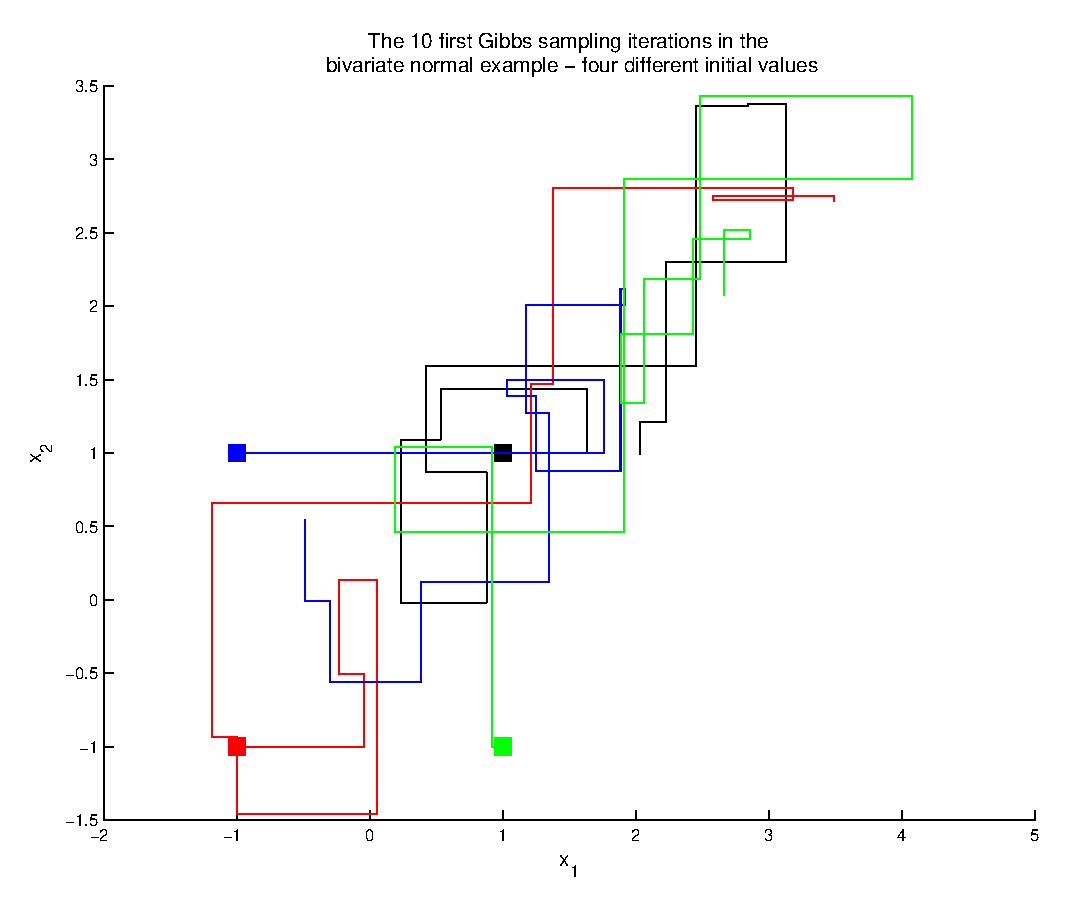
\includegraphics[scale=0.5,bb = 0 0 200 100, draft, type=eps]{../../BayesStat2011/Lectures/GibbsBivariateNormal1.eps}
%\par\end{center}
%
%\end{frame}
%
%%\begin{frame}{Gibbs sampling - Bivariate normal}
%%
%%
%%\begin{center}
%%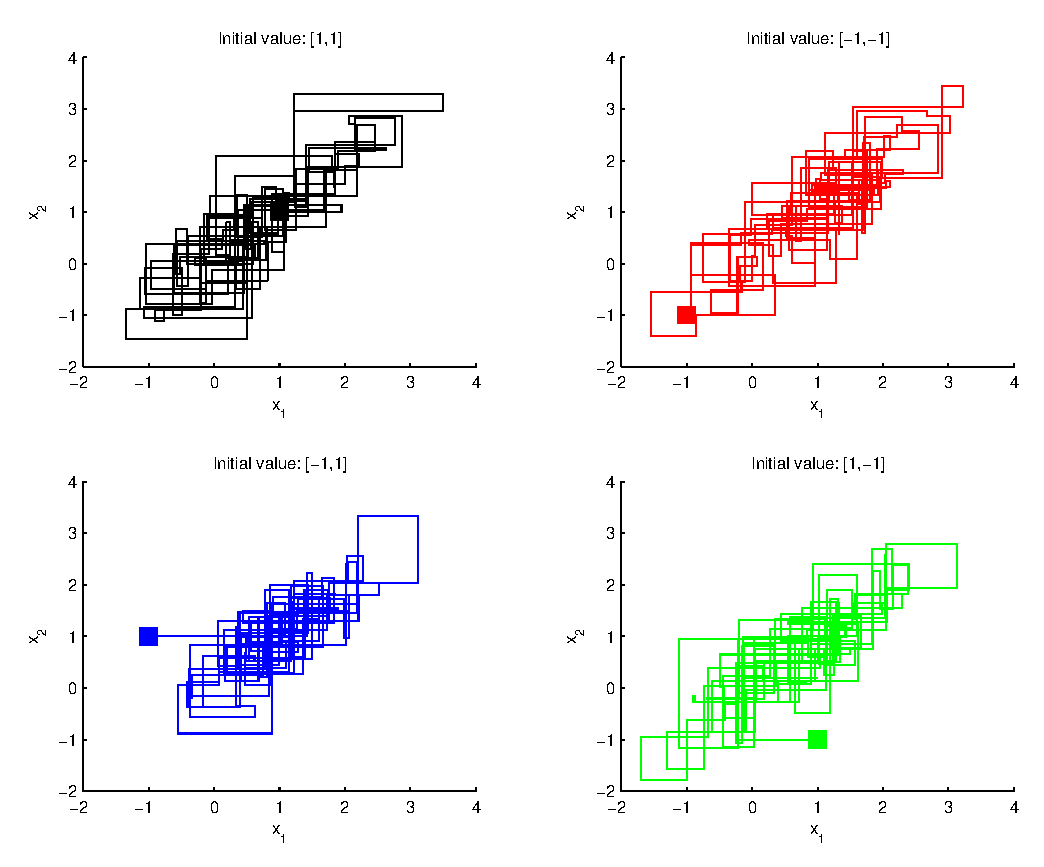
\includegraphics[scale=0.5,bb = 0 0 200 100, draft, type=eps]{../../BayesStat2011/Lectures/GibbsBivariateNormal2.eps}
%%\par\end{center}
%%
%%\end{frame}
%%
%%\begin{frame}{Gibbs sampling - Bivariate normal}
%%
%%
%%\begin{center}
%%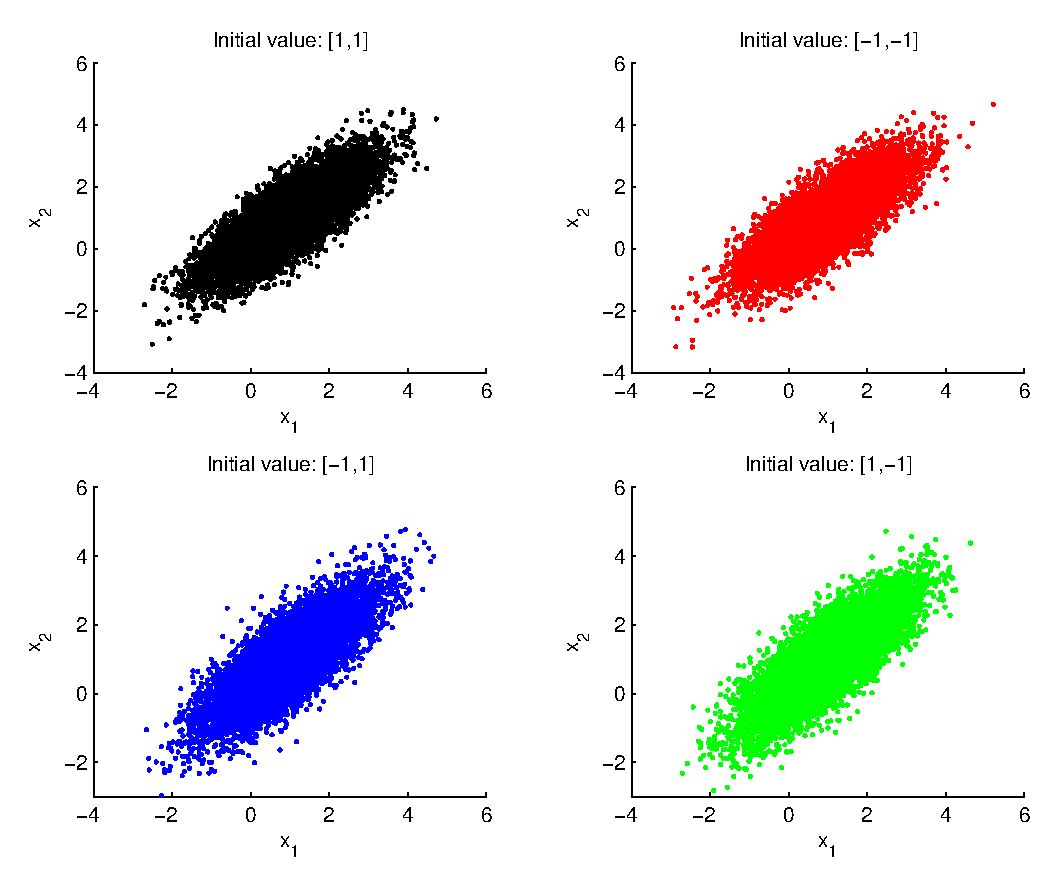
\includegraphics[scale=0.5,bb = 0 0 200 100, draft, type=eps]{../../BayesStat2011/Lectures/GibbsBivariateNormal3.eps}
%%\par\end{center}
%%
%%\end{frame}
%%
%%%\begin{frame}{Direct sampling vs Gibbs sampling}
%%
%%
%%\begin{center}
%%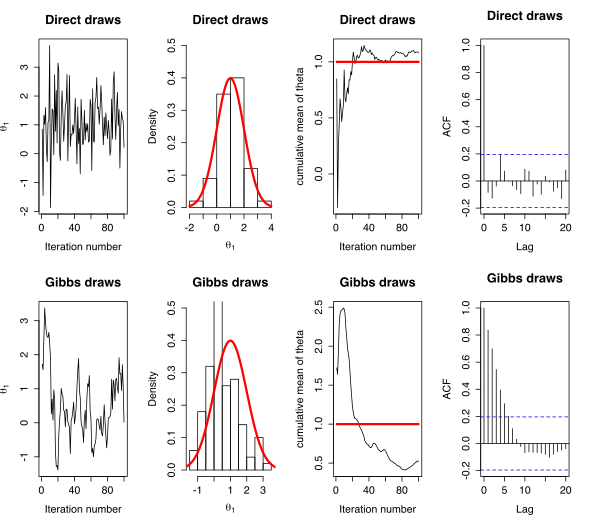
\includegraphics[scale=0.42]{DirectvsGibbs}
%%\par\end{center}
%%
%%\end{frame}
%%
%%\begin{frame}{Estimating the density of $g(\theta_{1},\theta_{2})=\sqrt{\theta_{1}^{2}+\theta_{2}^{2}}$}
%%
%%
%%\begin{center}
%%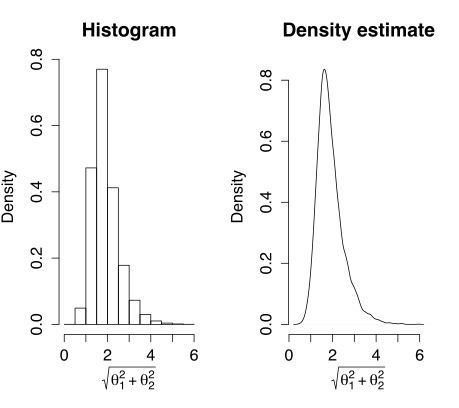
\includegraphics[scale=0.5]{EstLengthVector}
%%\par\end{center}
%%
%%\end{frame}
%
%%\begin{frame}{Estimating $Pr(\theta_{1}>0,\theta_{2}>0)$}
%%
%%\begin{itemize}
%%\item We can estimate a joint probability by counting: 
%%\[
%%Pr(\theta_{1}>0,\theta_{2}>0)\approx N^{-1}\sum_{i=1}^{N}1(\theta_{1}^{(i)}>0,\theta_{2}^{i)}>0)
%%\]
%% .
%%\end{itemize}
%%
%%\begin{center}
%%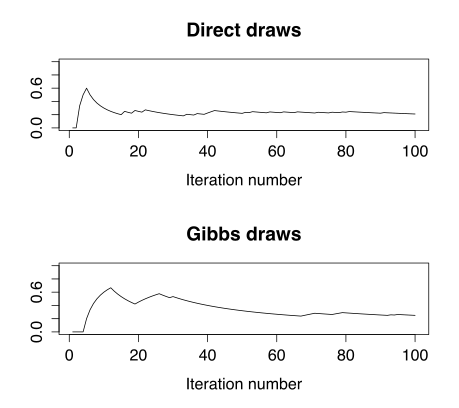
\includegraphics[scale=0.4]{CumsumJointProb}
%%\par\end{center}
%%
%%\end{frame}
%
%\begin{frame}{Gibbs sampling for normal model with non-conjugate prior}
%
%\begin{itemize}
%\item Normal model with semi-conjugate prior
%\begin{align*}
%\mu & \sim N(\mu_{0},\tau_{0}^{2})\\
%\sigma^{2} & \sim Inv-\chi^{2}(\nu_{0},\sigma_{0}^{2})
%\end{align*}
%
%\item Conditional posteriors
%\begin{align*}
%\mu|\sigma^{2},x & \sim N\left(\mu_{n},\tau_{n}^{2}\right)\\
%\sigma^{2}|\mu,x & \sim Inv-\chi^{2}\left(\nu_{n},\frac{\nu_{0}\sigma_{0}^{2}+\sum_{i=1}^{n}\left(x_{i}-\mu\right)^{2}}{n+\nu_{0}}\right)
%\end{align*}
%
%\end{itemize}
%\end{frame}
%
%\begin{frame}{Gibbs sampling for AR processes}
%
%\begin{itemize}
%\item \textbf{\textcolor{blue}{AR($p$) process}}
%\[
%x_{t}=\mu+\phi_{1}(x_{t-1}-\mu)+...+\phi_{p}(x_{t-p}-\mu)+\varepsilon_{t},\text{ \ \ }\varepsilon_{t}\overset{iid}{\sim}N(0,\sigma^{2}).
%\]
%
%\item Let $\phi=(\phi_{1},...,\phi_{p})'$.
%\item \textbf{\textcolor{blue}{Prior}}: 
%
%\begin{itemize}
%\item $\mu\sim$Normal
%\item $\phi\sim$Multivariate Normal
%\item $\sigma^{2}\sim$Scaled Inverse $\chi^{2}$.
%\end{itemize}
%\item The \textbf{\textcolor{blue}{posterior}} can be simulated by Gibbs
%sampling:
%
%\begin{itemize}
%\item $\mu|\phi,\sigma^{2},x\sim$ Normal
%\item $\text{\ensuremath{\phi}}|\mu,\sigma^{2},x\sim$ Multivariate Normal
%\item $\sigma^{2}|\mu,\phi,x\sim$ Scaled Inverse $\chi^{2}$ 
%\end{itemize}
%\end{itemize}
%\end{frame}
%
%\begin{frame}{Data augmentation - Mixture distributions }
%
%\begin{itemize}
%\item Let $\phi(x|\mu,\sigma^{2})$ denotes the \textbf{PDF} of a \textbf{normal}
%variable $x\sim N(\mu,\sigma^{2})$.\bigskip{}
%
%\item \textbf{\textcolor{blue}{Two-component mixture of normals}} {[}MN($2$){]}
%\[
%p(x)=\pi\cdot\phi(x|\mu_{1},\sigma_{1}^{2})+(1-\pi)\cdot\phi(x|\mu_{2},\sigma_{2}^{2})
%\]
%\medskip{}
%
%\item \textbf{\textcolor{blue}{Simulate}} from a MN($2$):
%
%\begin{itemize}
%\item Simulate an indicator $I\sim Bern(\pi)$.
%\item If $I=0$, simulate $x$ from $N(\mu_{1},\sigma_{1}^{2})$
%\item If $I=1$, simulate $x$ from $N(\mu_{2},\sigma_{2}^{2}).$
%\end{itemize}
%\end{itemize}
%\end{frame}
%
%\begin{frame}{Illustration of mixture distributions}
%
%
%\begin{center}
%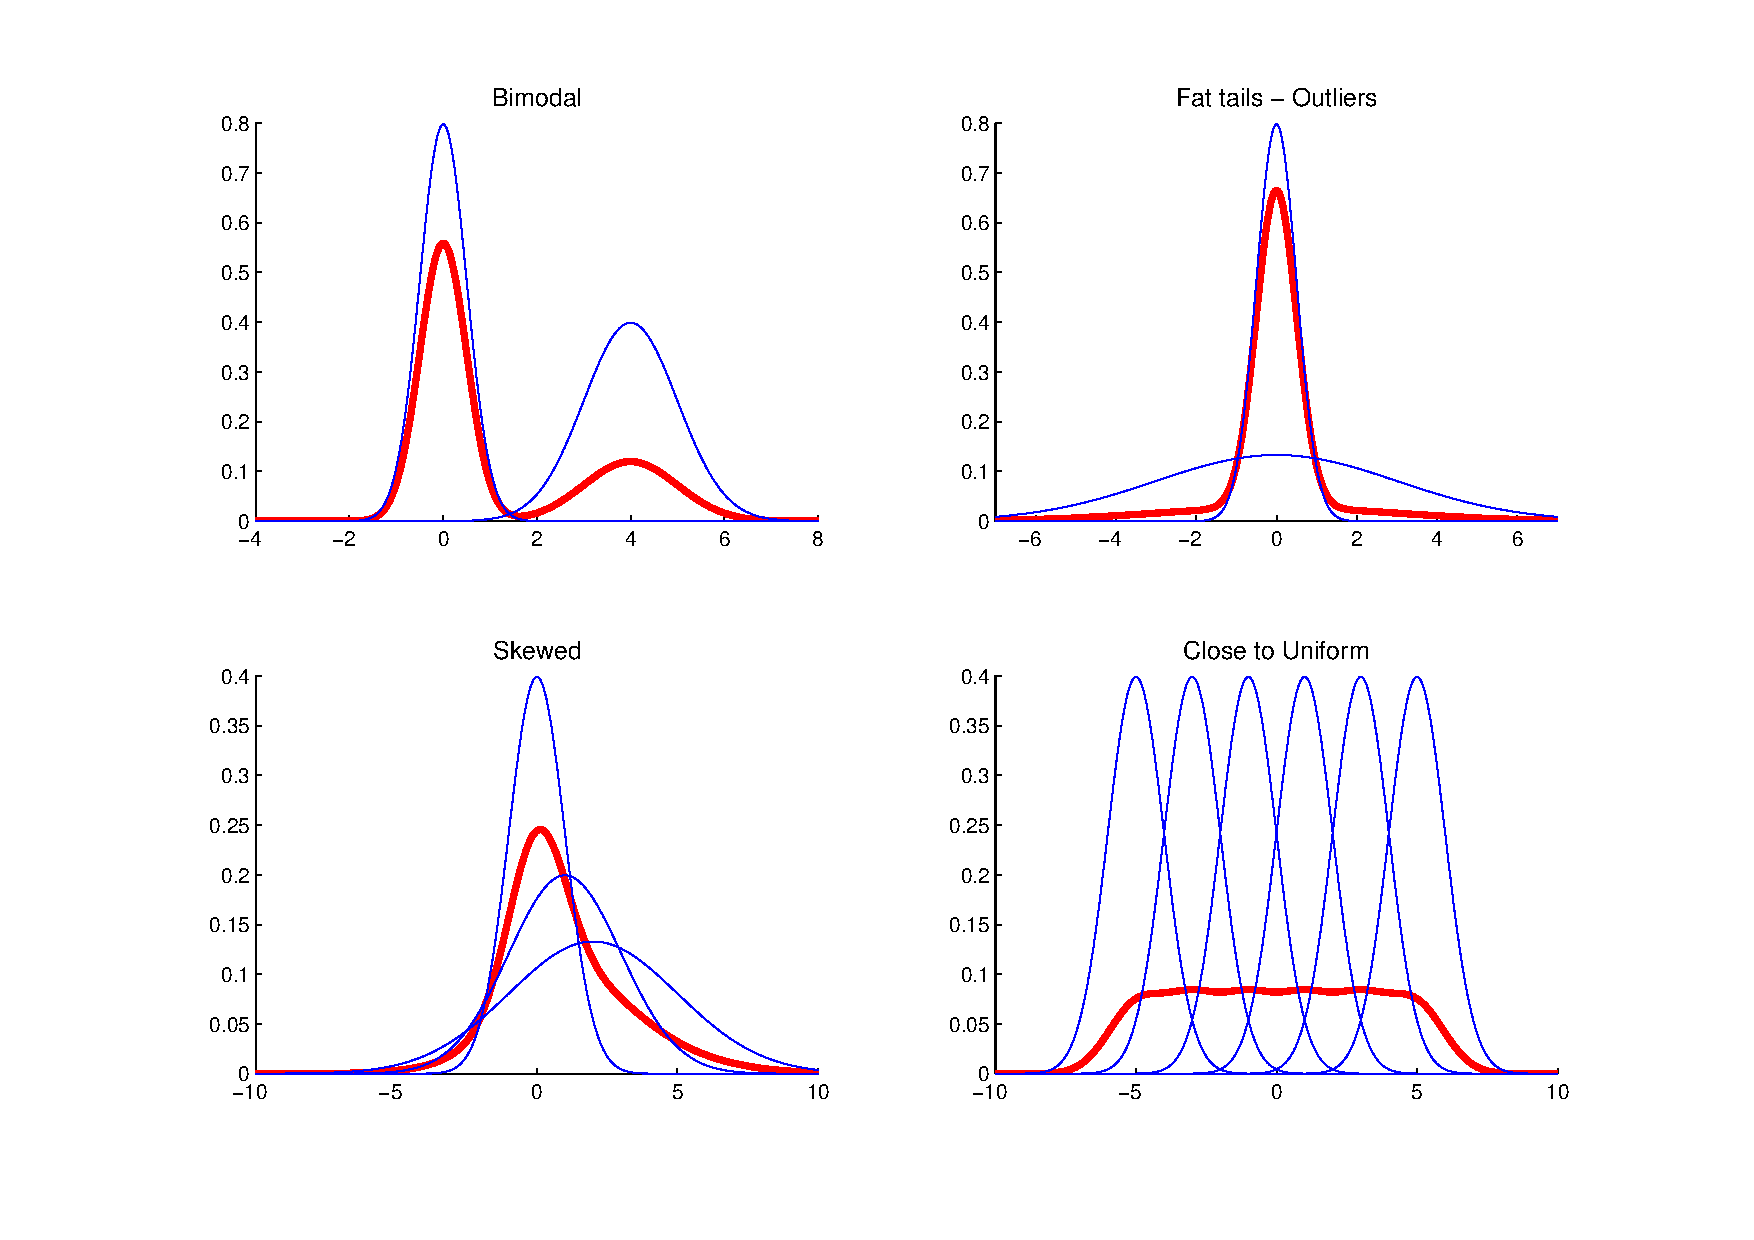
\includegraphics[scale=0.4,bb = 0 0 200 100, draft, type=eps]{../../BayesStat2011/Lectures/MixtureOfNormals.pdf}
%\par\end{center}
%
%\end{frame}
%
%\begin{frame}{Mixture distributions, cont.}
%
%\begin{itemize}
%\item Not easy to estimate directly - the likelihood is a product of sums.
%\item \textbf{Assume} that we knew which of the two densities each observation
%came from. 
%\[
%I_{i}=\left\{ \begin{array}{c}
%0\text{ if }x_{i}\text{ came from Density 1}\\
%1\text{ if }x_{i}\text{ came from Density 2}
%\end{array}\right..
%\]
%
%\item Armed with knowledge of $I_{1},...,I_{n}$ it is now easy to estimate
%$\pi$, $\mu_{1},\sigma_{1}^{2},\mu_{2},\sigma_{2}^{2}$ by separating
%the sample according to the $I$'s.
%\item But we do \textbf{not} know $I_{1},...,I_{n}$!
%\end{itemize}
%\end{frame}
%
%\begin{frame}{Mixture distributions, cont.}
%
%\begin{itemize}
%\item Gibbs sampling to the rescue. 
%\item Assume: Prior $\pi$ $\sim Beta(\alpha_{1},\alpha_{2})$. Conjugate
%prior for $(\mu_{j},\sigma_{j}^{2}),$ see Lecture 3. $n_{2}=\sum\nolimits _{i=1}^{n}I_{i}$
%and $n_{1}=n-n_{2}$.
%\item Algorithm:
%
%\begin{itemize}
%\item $\pi$ $|$ $I,x\sim Beta(\alpha_{1}+n_{1},\alpha_{2}+n_{2})$
%\item $\sigma_{1}^{2}$ $|$ $I,x\sim Inv$-$\chi^{2}$ and $\mu_{1}|I,\sigma_{1}^{2},x\sim N$
%\item $\sigma_{2}^{2}$ $|$ $I,x\sim Inv$-$\chi^{2}$ and $\mu_{2}|I,\sigma_{2}^{2},x\sim N$
%\item $I_{i}$ $|$ $\pi,\mu_{1},\sigma_{1}^{2},\mu_{2},\sigma_{2}^{2},x\sim Bern(\theta_{i})$,
%$i=1,...,n,$
%\[
%\theta_{i}=\frac{(1-\pi)\phi(x_{i};\mu_{2},\sigma_{2}^{2})}{\pi\phi(x_{i};\mu_{1},\sigma_{1}^{2})+(1-\pi)\phi(x_{i};\mu_{2},\sigma_{2}^{2})}.
%\]
% 
%\end{itemize}
%\end{itemize}
%\end{frame}
%
%\begin{frame}{Mixture distributions, cont.}
%
%\begin{itemize}
%\item \textbf{\textcolor{blue}{$K$-component mixture of normals}}
%\[
%p(x)=\sum_{k=1}^{K}\pi_{k}\phi(x;\mu_{k},\sigma_{k}^{2}),
%\]
%where $\sum\nolimits _{k=1}^{K}\pi_{k}=1$.
%\item \textbf{Multi-class indicators}: $I_{i}=k$ if observation $i$ comes
%from density $k$.
%\item \textbf{\textcolor{blue}{Gibbs sampling}} with 
%
%\begin{itemize}
%\item $(\pi_{1},...,\pi_{K})$ $|$ $I,x\sim Dirichlet(\alpha_{1}+n_{1},\alpha_{2}+n_{2},...,\alpha_{K}+n_{K})$
%\item $\sigma_{k}^{2}$ $|$ $I,x\sim Inv$-$\chi^{2}$ and $\mu_{k}|I,\sigma_{k}^{2},x\sim Normal$,
%\ \ $for$ $k=1,...,K,$
%\item $I_{i}$ $|$ $\pi,\mu,\sigma^{2},x\sim Multinomial(\theta_{i1},...,\theta_{iK})$,
%$for$ $i=1,...,n,$
%\[
%\theta_{ij}=\frac{\pi_{j}\phi(x_{i};\mu_{j},\sigma_{j}^{2})}{\sum_{r=1}^{k}\pi_{r}\phi(x_{i};\mu_{r},\sigma_{r}^{2})}.
%\]
%
%\end{itemize}
%\item Gibbs sampling is very powerful for \textbf{\textcolor{blue}{missing
%data}} problems. \textbf{\textcolor{blue}{Semi-supervised learning}}.
%\end{itemize}
%\end{frame}
%
%\begin{frame}{Data augmentation - Probit regression}
%
%\begin{itemize}
%\item \textbf{\textcolor{blue}{Probit}} model:
%\[
%\Pr(y_{i}=1\text{ }|\text{ }x_{i})=\Phi(x_{i}^{\prime}\beta)
%\]
%
%\item \textbf{\textcolor{blue}{Random utility formulation}} of the probit:
%\begin{eqnarray*}
%u_{i} & \sim & N(x_{i}^{\prime}\beta,1)\\
%y_{i} & = & \left\{ \begin{array}{c}
%1\text{ \ \ om }u_{i}>0\\
%0\text{ \ \ om }u_{i}\leq0
%\end{array}.\right.
%\end{eqnarray*}
%
%\item Check: $\Pr(y_{i}=1$ $|$ $x_{i})=\Pr(u_{i}>0)=1-\Pr(u_{i}\leq0)=1-\Pr(u_{i}-x_{i}^{\prime}\beta<-x_{i}^{\prime}\beta)=1-\Phi(-x_{i}^{\prime}\beta)=\Phi(x_{i}^{\prime}\beta)$.
%\item If $u=(u_{1},...,u_{n})$ were observed, then $\beta$ could be analyzed
%by traditional linear regression. But, $u$ is \textbf{not observed}.
%Gibbs sampling to the rescue!
%\end{itemize}
%\end{frame}
%
%\begin{frame}{Gibbs sampling for the Probit regression}
%
%\begin{itemize}
%\item Simulate from joint posterior $p(u,\beta|y)$ iterating between the
%\textbf{\textcolor{blue}{full conditional posteriors}}: 
%
%\begin{itemize}
%\item \textrm{$p(\beta|u,y)$, which is multivariate normal (this is just
%a linear regression)}
%\item \textrm{$p(u_{i}|\beta,y),\text{ }i=1,...,n$.}
%\end{itemize}
%\item The full conditional posterior distribution of $u_{i}$ is: 
%\begin{align*}
%p(u_{i}|\beta,y) & \propto p(y_{i}|\beta,u_{i})p(u_{i}|\beta)\\
% & =\begin{cases}
%N(u_{i}|x_{i}^{\prime}\beta,1) & \text{truncated to }u_{i}\in(-\infty,0]\text{ if }y_{i}=0\\
%N(u_{i}|x_{i}^{\prime}\beta,1) & \text{truncated to }u_{i}\in(0,\infty)\text{ if }y_{i}=1
%\end{cases}
%\end{align*}
%
%\item Collect the $\beta$-draws. A histogram of these draws approximates
%$p(\beta|y)=$ $\int p(u,\beta|y)du$.
%\end{itemize}
%\end{frame}
%
%\begin{frame}{Improving the efficiency of the Gibbs sampler}
%
%\begin{itemize}
%\item \textbf{\textit{\textcolor{blue}{\emph{Efficient blocking}}}}. Correlated
%parameters should ideally be included in the same updating block.\bigskip{}
%
%\item \textbf{\textit{\textcolor{blue}{\emph{Reparametrization}}}}. Convergence
%can improve dramatically in alternative parametrizations.\bigskip{}
%
%\item \textbf{\textit{\textcolor{blue}{\emph{Data augmentation}}}}. Bring
%in latent (unobserved) variables that make the full conditional posteriors
%more easily sampled (Probit, Mixture models etc). Downside: Typically
%increases the autocorrelation between draws.\bigskip{}
%
%\item \textbf{\textit{\textcolor{blue}{\emph{Parameter expansion}}}}. Introducing
%(non-sense) parameters in the model may break the dependence between
%the original parameters (Example probit).\end{itemize}
%\end{frame}
%
%
%\begin{frame}
%\frametitle{References}
%\small{
%\textbf{Andrew, G., Carlin, J., Stern, H., Dunson, D., Vehtari, A., and Rubin, D. (2014)}. Bayesian data analysis, Third edition.}
%
%%\addcontentsline{toc}{section}{\refname}\bibliography{ref}
%\end{frame}
%
%
%







\end{document}

